% !TEX root=../main.tex
\section{Experimental Setup}
\label{sec:ocnn_experiment-setup}

In this section, we show the empirical effectiveness of OC-NN formulation over the state-of-the-art methods on real-world data. Although our method is applicable in any context where autoencoders may be used for feature representation, e.g., speech.  Our primary focus will be on non-trivial high dimensional images.
%\vspace{-0.3 cm}
\subsection{Methods compared}
\label{sec:methods_compared}
We compare our proposed one-class neural networks (OC-NN) with the following state-of-the-art methods for anomaly detection:
\let\labelitemi\labelitemii
\begin{itemize}{}
	\item \textbf{OC-SVM -SVDD} as per formulation in ~\cite{scholkopf2002support}
    \item \textbf{Isolation Forest} as per formulation in ~\cite{liu2008isolation}.
	\item \textbf{Kernel Density Estimation (KDE)} as per formulation in ~\cite{parzen1962estimation}.
    \item \textbf{Deep Convolutional Autoencoder (DCAE)} as per formulation in ~\cite{masci2011stacked}.
    \item \textbf{AnoGAN} as per formulation in ~\cite{radford2015unsupervised}.
    \item \textbf{Soft-Bound and One Class Deep SVDD} as per formulation in ~\cite{pmlrv80ruff18a}.
    \item \textbf{Robust Convolutional Autoencoder (RCAE)} as per formulation in ~\cite{chalapathy2017robust}.
	\item \textbf{One-class neural networks (OC-NN) \footnote{\url{https://github.com/raghavchalapathy/oc-nn}}}, our proposed model as per Equation \ref{eqn:oc-nn}.
\end{itemize}
We used Keras~\cite{chollet2015keras} and  TensorFlow~\cite{abadi2016tensorflow} for the implementation of OC-NN, DCAE, RCAE \footnote{\url{https://github.com/raghavchalapathy/rcae}}
For OC-SVM\footnote{\url{http://scikit-learn.org/stable/auto_examples/svm/plot_oneclass.html}} and Isolation Forest\footnote{\url{http://scikit-learn.org/stable/modules/generated/sklearn.ensemble.IsolationForest.html}}, we used publicly available implementations.

\begin{table}[!t]
    \centering
    \renewcommand{\arraystretch}{1.25}
    \setlength{\tabcolsep}{6pt}
    %\scalebox{0.85}{
    \begin{tabular}{@{}llll@{}}
        \toprule
        \toprule
        Dataset & \# instances & \# anomalies & \# features \\
        \toprule
        {\tt Synthetic}       & 190   & 10                                        & 512 \\
        {\tt MNIST}           & single class   & 1\%  ( from all class)            & 784 \\
        {\tt CIFAR$-$10}      & single class    & 10\% ( from all class)           &3072 \\
        {\tt GTSRB }           & 1050 (stop signs )     & 100 (boundary attack)  &3072 \\
        \bottomrule
    \end{tabular}
    %}
    %\vspace{0.1 cm}
    \caption{Summary of datasets used in experiments.}
    \label{tbl:datasets}
    \vspace{-\baselineskip}
\end{table}

% \vspace{-0.5 cm}
\subsection{Datasets}
%%\vspace{-0.2 cm}
We compare all methods on synthetic and four real-world datasets as summarized below :
\begin{itemize}
	\item {\tt Synthetic Data}, consisting of 190 normal data points 10 anomalous points drawn from normal distribution with dimension $512$.
	\item {\tt MNIST}, consisting of 60000 $28\times28$ grayscale images of handwritten digits  in 10 classes, with 10000  test images~\cite{lecun2010mnist}.
	\item {\tt GTSRB }, are $32\times32$ colour images comprising of  adversarial boundary attack on stop signs boards~\cite{stallkamp2011german}.
	\item {\tt CIFAR$-$10} consisting of 60000 $32\times32$ colour images in 10 classes, with 6000 images per class~\cite{krizhevsky2009learning}.
\end{itemize}

For each dataset, we perform further processing to create a well-posed anomaly detection task, as described in the next section.
\vspace{-0.3 cm}

\subsection{Evaluation of Models}
\label{sec:evaluationOfModels}
% Shallow methods compared
\subsubsection{\textbf{Baseline Model Parameters:}}
\label{sec:baselinemodel_parameters.}
The proposed OC-NN method is compared with several state-of-the-art baseline models as illustrated in Table~\ref{tab:ocnn_results}. The model parameters of shallow baseline methods are used as per implementation in~\cite{pmlrv80ruff18a}. Shallow Baselines (i) Kernel OC-SVM/SVDD with
Gaussian kernel. We select the inverse length scale $\gamma$ from
$\gamma$  $\in$ {$2^{ - 10}$ , $2^{ - 9}$, . . . , $2^{ - 1}$ via grid search using the performance on a small holdout set (10) \% of randomly drawn test samples). We run all experiments for $\nu = 0.1$ and report the better result. (ii) Kernel density estimation (KDE). We select the bandwidth \textit{h} of the Gaussian kernel from \textit{h} $ \in {2^{0.5} , 2 ^1, . . . , 2^5}$ via 5-fold cross-validation using  the log-likelihood score. (iii) For the  Isolation Forest (IF) we set the number of trees to \textit{t} = 100 and the sub-sampling size to $\Psi = 256$, as recommended in the original work~\cite{pmlrv80ruff18a}.
\vspace{-0.4cm}
% Deep Anomaly detection models compared
\subsubsection{ \textbf{Deep Baseline Models:}}
We compare OC$-$NN models to  four deep approaches described Section ~\ref{sec:methods_compared}.
We choose to train DCAE using the Mean sqaure error (MSE) loss since our experiments are on image data. For the DCAE encoder, we employ the same network architectures as we use for Deep SVDD, RCAE, and OC-NN models. The decoder is then constructed symmetrically, where we substitute max-pooling with upsampling. For AnoGAN we follow the implementation as per ~\cite{radford2015unsupervised} and set
the latent space dimensionality to $256$.
For we Deep SVDD, follow the implementation as per ~\cite{pmlrv80ruff18a} and employ a  two phase learning rate schedule (searching + fine tuning) with initial learning rate $\eta$ = $10^{ - 4}$  and subsequently $\eta$ = $10^{ - 5}$. For DCAE we train 250 + 100 epochs, for Deep SVDD 150 + 100. Leaky ReLU activations are used with leakiness $\alpha=0.1$. For RCAE we train the autoencoder using the robust loss and follow the parameter settings as per formulation in ~\cite{chalapathy2017robust}.

%OC-NN Model Architecture proposed
\subsubsection{ \textbf{One-class neural Networks (OC-NN):}}
\label{model_architecture}
In OC-NN technique firstly, a deep autoencoder is trained to obtain the representative features of the input as illustrated in Figure~\ref{fig:model-architecture}(a). Then, the encoder layers of this pre-trained autoencoder is copied and fed as input to the feed-forward network with one hidden layer as shown in Figure~\ref{fig:model-architecture}(b). The summary of feed forward network architecture's used for various datasets is presented in Table~\ref{tbl:feed-forward-OC-NN}. The weights of encoder network are not frozen (but trained) while we learn feed-forward network weights, following the algorithm summarized in Section~\ref{sec:algorithm}. A feed-forward neural network consisting of single hidden layer, with  linear activation functions produced the best results, as per Equation~\ref{eqn:oc-nn}.  The optimal value of parameter $\nu$ $\in$ ${[0, 1]}$ which is equivalent to the percentage of anomalies for each data set, is set according to respective outlier proportions.

% \vspace{-0.2cm}
% Model architectures tested
% \begin{figure*}
% \subfloat[Autoencoder .\label{sfig:autoencoder-for-representation-learning}]{%
%   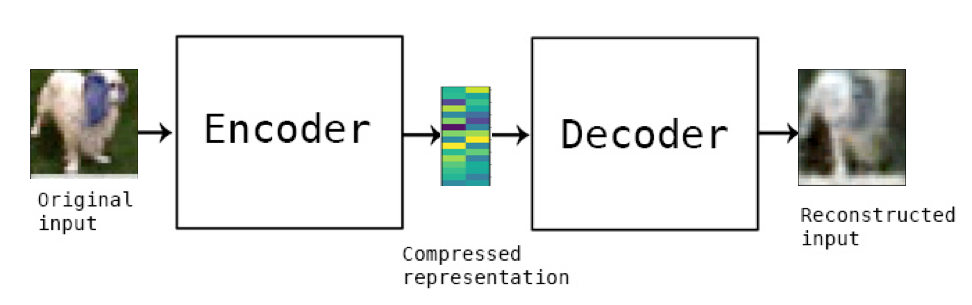
\includegraphics[width=.40\linewidth]{images/transferLearningAE}%
% }\hspace{0.5cm}
% \subfloat[one-class neural networks. \label{sfig:oc-nn-model-architecture}]{%
%   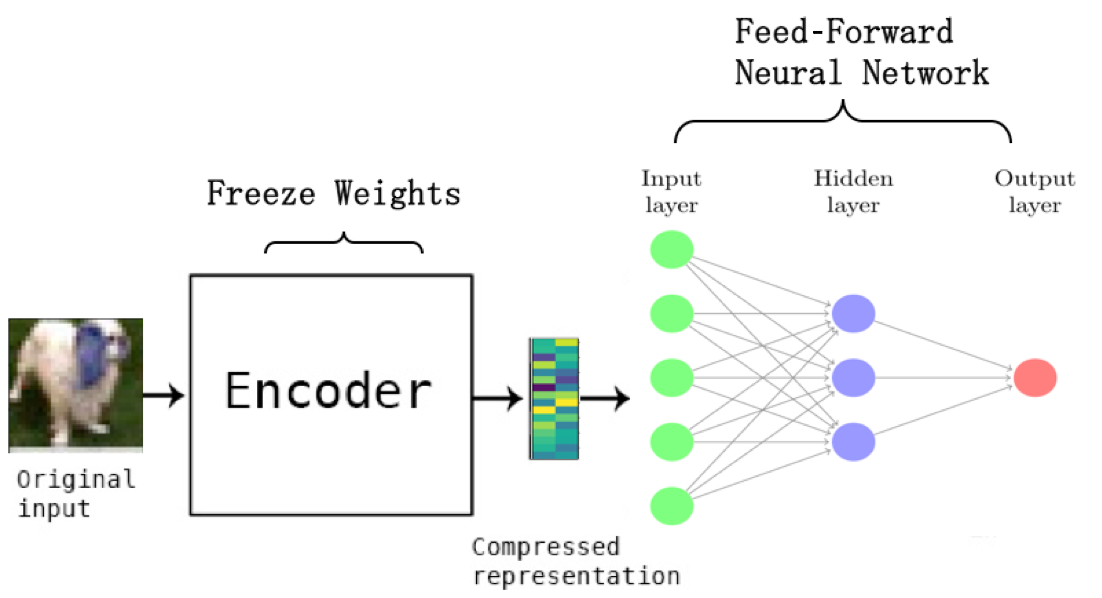
\includegraphics[width=.40\linewidth]{images/oneClassNN_model}%
% }
% \caption{Model architecture of Autoencoder  and the proposed one-class neural networks (OC-NN).}
% \label{fig:model-architecture}
% \end{figure*}
% %  End of the Figure

\begin{figure}[!t]
     \begin{subfigure}[b]{1\textwidth}
   \centering
   {\includegraphics[scale=0.50]%{catswithrotatedcats}}
{images/transferLearningAE}}
\caption{Autoencoder.}
        \end{subfigure}%
        \hfill
        \vspace{2mm}
     \begin{subfigure}[b]{1\textwidth}
\centering
   {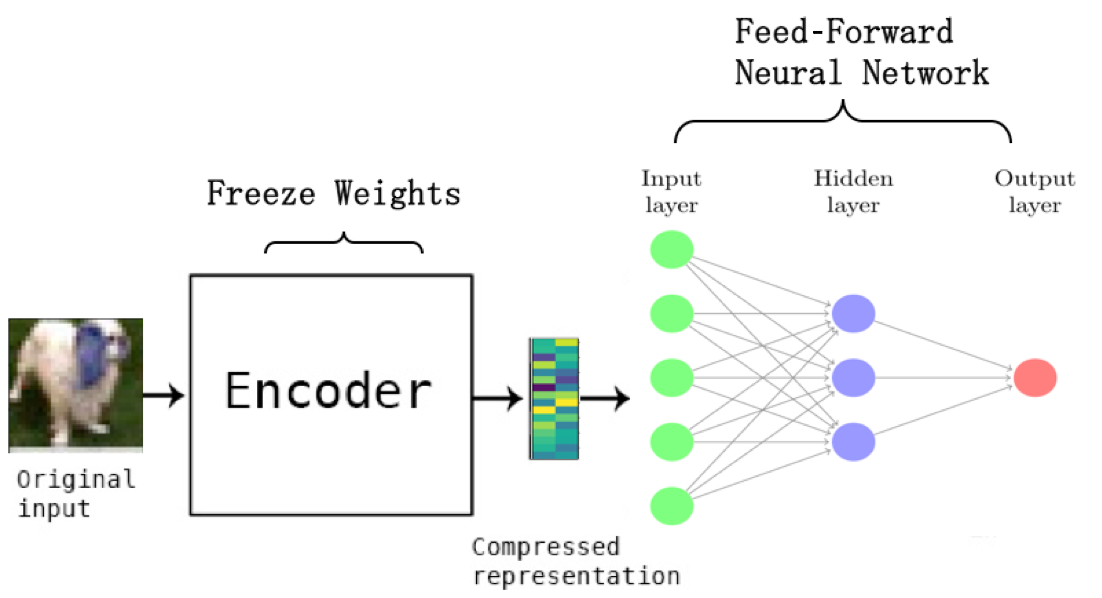
\includegraphics[scale=0.50]{images/oneClassNN_model}}
 \caption{One-class neural networks.}
        \end{subfigure}%
    \caption{
     Model architecture of Autoencoder  and the proposed one-class neural networks (OC-NN).
    }
    \label{fig:model-architecture}
\end{figure}




%Table containing the feed forward network architectures used in experiments
\begin{table}[!t]
    \centering
    \renewcommand{\arraystretch}{1.25}
    \setlength{\tabcolsep}{6pt}
    %\scalebox{0.85}{
    \begin{tabular}{@{}llll@{}}
        \toprule
        \toprule
         Dataset& \#    Input (features) & \# hidden layer( or output) \# optional layer  \\
        \toprule
        {\tt Synthetic }      & 512     & 128   & 1 \\
        {\tt MNIST}           & 32      & 32    & None \\
        {\tt CIFAR$-$10}      & 128     & 32    & None \\
        {\tt GTSRB }          & 128     & 32    & 16 \\
        \bottomrule
    \end{tabular}
    %}
    %\vspace{0.1 cm}
    \caption{Summary of best performing feed-forward network architecture's used in OC-NN model for experiments.}
    \label{tbl:feed-forward-OC-NN}
    \vspace{-\baselineskip}
\end{table}
% end of the table

































